%-*- program: pdflatex -*-
%-*- program: bibtex -*-
%-*- program: pdflatex -*-
%-*- program: pdflatex -*-


% --------------------------------------------------------------
% Preamble
% --------------------------------------------------------------

\documentclass{article}
\usepackage{arxiv}
\usepackage[utf8]{inputenc} % allow utf-8 input
\usepackage[T1]{fontenc}    % use 8-bit T1 fonts
\usepackage{hyperref}       % hyperlinks
\usepackage{url}            % simple URL typesetting
\usepackage{xcolor}
\hypersetup{
    colorlinks,
    linkcolor={red!50!black},
    citecolor={blue!50!black},
    urlcolor={blue!80!black}
}
\usepackage{booktabs}       % professional-quality tables
\usepackage{tabularx}
\usepackage{amsfonts}       % blackboard math symbols
\usepackage{nicefrac}       % compact symbols for 1/2, etc.
\usepackage{microtype}      % microtypography
\usepackage{gensymb}        % degree, angle symbols

% for math equations and symbols
\usepackage{amsmath} 
\usepackage{amssymb} 
\newcommand{\E}{\mathbb{E}}
\newcommand{\SD}{\mathit{SD}}
\newcommand{\SE}{\mathit{SE}}
\newcommand{\BF}{\mathit{BF}}
\DeclareMathOperator\arctanh{arctanh}

% This prevents placing floats before a section.
\usepackage{placeins}

% bibliography
\usepackage{natbib}


%%% some support for commenting

\usepackage{color}
\definecolor{Blue}{RGB}{0,0,255}
\definecolor{Red}{RGB}{255,0,0}
\newcommand{\jo}[1]{\textcolor{Red}{[Jacob: #1]}}  
\newcommand{\hs}[1]{\textcolor{Blue}{[Hrvoje: #1]}} 
% \newcommand{\jo}[1]{}  
% \newcommand{\hs}[1]{} 


% ---------------------------------------------------------
% Title, authors
% ---------------------------------------------------------

\title{A meta-analysis of eye movements in decision-making}

% Alternatives
% The visual environment influences attention during decision making
% Visual environments, attention and decision making
% A meta analysis of influence of the visual environement factors on  attention in decision making

\author{
  Jacob L. Orquin\thanks{Correspondence concerning this article should be addressed to Jacob L. Orquin, Department of Management/MAPP, Aarhus University, Fuglesangs alle 4, 8210 Aarhus V - Denmark. E-mail: jalo@mgmt.au.dk. Data and scripts are available at: \url{https://osf.io/buk7p/}. This research was supported by the Independent Research Fund Denmark, grant number: 8046-00014A. The authors thank Martin Meissner, Tobias Otterbring, Sonja Perkovic, and Valdimar Sigurdsson for feedback on earlier versions of the manuscript.}, Erik S. Lahm, Hrvoje Stojić
}


\begin{document}
\maketitle

% ---------------------------------------------------------
% Abstract
% ---------------------------------------------------------


\begin{abstract}  % NHB limit: 150 words
As decision-makers, we rely on our eyes for gathering information in a vast number of tasks every day. A growing body of research attempts to understand what drives eye movements in decision-making and how eye movements are related to the decision process. Different models have been proposed, assuming that eye movements are driven separately or in combination by either by goal related top-down factors or stimulus related bottom-up factors. We meta-analyze empirical studies on eye movements in decision-making and provide a quantitative overview of some of the factors driving eye movements. Our findings reveal that the bottom-up factors, salience ($\rho = .13$), surface size ($\rho = .38$), left vs right positioning ($\rho = .27$), central positioning ($\rho = .43$), and set size ($\rho = .28$), all influence what decision-makers gaze at independently of the decision task or preferences. Top-down factors have a slightly larger effect on eye movements than bottom-up factors: decision-makers gaze more at information that is relevant in terms of task goals ($\rho = .42$) or subjective preferences ($\rho = .48$) and gaze more at the eventually chosen option ($\rho = .70$) regardless of whether the choice is based on preferences or inferences. Our findings show a need for incorporating bottom-up factors in models that jointly explain eye movements and decision-making.
\end{abstract}

\keywords{eye movements, decision-making, meta-analysis, top-down control, bottom-up control} 


% -------------------------------------------------------
% Introduction
% -------------------------------------------------------

\section{Significance statement}

In decision making we often gather information with our eyes. We show that decision makers are more likely to gaze at information that is relevant to the decision task or their preferences, but also gaze more at information when it is salient, large, centrally positioned, and uncluttered independently of its relevance. Because the structure of our visual environment plays a large role in determining eye movements, citizens and policy makers should be aware of who is in control of the visual environment and how it can bias information processing in favor of or against the interests of decision makers.   


% \section{Motivation and Problem}

Decision making often takes place in environments where relevant information needs to be acquired visually. In such visual environments options can differ in their position, surface size, salience and many other visual properties. Consider encountering a product with surprising color on a  supermarket shelf, or a restaurant menu where items either have or do not have an accompanying picture. Such visual properties have been shown to influence our attention during decision making in real world situations and there is now substantial evidence showing that attention plays an important role in decision making \cite{gidloef2017a}, and can even causally affect choices (Krajbich 2013 PNAS paper; Shimojo 2003; ...). However, the role of visual properties is almost completely absent from prominent decision making theories. In most theories, the decision task determines the relevance of objects and, either explicitly or implicitly, whether and when we look at them. Here, we ask whether decision research is building on correct assumptions about visual attention and the role of the visual environment and provide an empirical assay of the relative importance of various visual and task factors to guide further theory development.


% \section{Decision research (mostly) ignores bottom-up factors}

Most decision research considers attention to be determined by the decision process, that it is driven by the goal relevance of objects rather than the visual properties of these objects. In many prominent decision making models this assumption is implicit. Consider, for example, the prospect theory model of how probabilities and values of options are integrated  to arrive at a preferential choice (Kahneman Tversky 79). Options are treated equally according to this model, and nothing in the model indicates that one piece of information would attract more attention than the other. Prospect theory and other related variants of expected utility theory are focused on capturing the final choices, not the process of how people arrive at choices, which one could argue is more important for attention. However, popular process-oriented decision making models commit to similar assumptions about attention. Consider, for example, satisficing, elimination-by-aspect, or the lexicographic heuristics (Goldstein, Gigerenzer 1996; Bettman, Payne, Johnson 1988; Simon, 1956, Tversky, 1976). While these models all specify different information search processes, they make similar implicit assumptions about the nature of visual search and hence attention in decision making. These  models assume that the information search is determined by a search rule inherent to the decision process, e.g. attend to options one at a time until a satisfactory option is found (satisficing: Stüttgen et al., 2012), or attend to information cues in order of their validity until a cue is found that identifies the best option (lexicographic: Krefeld-Schwalb, Rosner 2019). Correspondingly, in experiments evaluating these models care is usually taken that visual factors have been controlled for – options have the same size and salience, their locations are carefully counterbalanced and so on. 

In sequential sampling models of decision making attention has had a more explicit role. Sequential sampling models assume that stochastic evidence for an alternative is accumulated over time and when the integrated evidence reaches a threshold a choice is made. This is a process-oriented model that aims to capture how people balance the value of accumulating more information with the cost of taking more time to reach a decision (Ratcliff for DDM; Brown etal 2010 for LBA). In two influential variants of these models attention plays an important role, by determining how evidence is sampled in favor of choice options (DFT) or by determining the weight assigned to the evidence (aDDM). In these models attention, fluctuates randomly between choice options or choice attributes until a choice is made. The implicit assumption being, that in the long run attention is uniformly distributed over options and attributes. This is a stochastic equivalent to a maximizing decision rule such as the weighted additive which assumes that a decision maker attends equally to all information (Glöckner, Schulte). In other words, even though attention exerts influence on choices, this influence is random and neither controlled by goals or the visual environment. Recently, sequential sampling models have been proposed in which attention is guided by the value of choice options (Callaway \& Griffiths, 2019; Gluth et al., 2019). This assumption is supported by empirical findings demonstrating value based attentional capture, i.e. the effect that objects associated with rewards capture attention (Le Pelley et al., 2015). The models are reminiscent of an earlier idea by Shimojo and colleagues (2003) who proposed that decision makers attend preferentially to high value options, which increases their value further, thus creating a feedback loop and increasing likelihood of gazing at the ultimately chosen option. 

There are a few studies that proposed decision making models where attention is not driven only by the goal relevance of options, but also by their visual properties, focusing on visual salience. For example, Towal and colleagues (2013) showed that visual salience continuously influences the decision process by making some choice options more likely to attract fixations, but does not influence the drift rate towards salient choice options directly. Chen and colleagues (REF) provided evidence that salience can determine the onset of drift towards a choice option, but not the drift rate itself. Finally, Navalpakkam and colleagues (2010) showed that decision makers in a reward harvesting task made choices by combining value and visual salience, consistent with an ideal Bayesian observer. This work suggests that salience can influence the decision process directly rather than by biasing attention, and, through that, the onset or amount of drift. 


% \section{Why do we need bottom up factors in decision making models?}

The assumption in decision science about cognitive factors driving attention in decision making is inconsistent with a number of findings. Wedel and Pieters (REF), for instance, suggest that 1/3 of variance in attention is due to factors in the visual environment, unrelated to the decisions task, and Towal and colleagues propose a similar ratio of cognitive vs stimulus factors (REF). There are also several model free studies showing simultaneous and additive effects of cognitive and visual factors \cite{gidloef2017a,orquin2015a,peschel2019}. Moreover, there is evidence that the visual environment influence choices by biasing visual attention. For instance, decision irrelevant visual factors have been shown to influence time preferences \cite{reeck2017a}, risk preferences (Fisher), and consumer preferences (Orquin).

Further evidence comes from vision science research. The few studies that modelled the influence of the visual environment on attention in decision making focused exclusively on salience (towal, chen, Navalpakkam). This focus is justified - in terms of bottom-up control a great deal of research in vision science has concentrated on visual salience (for a review see Borji \& Itti, 2012). The term visual salience refers to the stimuli that differ from their surroundings in terms of visual conspicuity and it is assumed that observers are more likely to gaze at stimuli that are high in visual salience. Models of visual salience typically assume that the visual cortex computes a topographic salience map that guides attention selection (Itti \& Koch, 2000), based on various visual aspects such as color, contrast, or movement (Itti \& Koch, 2001). There are at least three other bottom-up factors that are likely to be particularly relevant in decision making setting. First factor is the relative surface size of stimuli, which refers to the proportion of the visual environment occupied by the stimulus (for a review see Peschel \& Orquin, 2013). The effect of surface size is most likely a consequence of the psychophysical properties of the visual system (Dehaene, 2003), since increments of the surface size exhibit a diminishing marginal increase on eye movements (Lohse, 1997). While surface size is typically controlled in laboratory decision studies, in natural decision situations surface size varies substantially (Orquin et al., 2019). A second factor is the position of stimuli which has been shown to influence eye movements and is typically corrected for in vision research models when estimating the influence of other variables of interest (Clarke \& Tatler, 2014). In decision making context options typically come in different spatial locations, which means that position effects like left-to-right (reading) direction and centrality are likely to hold (Chandon et al., 2009; Atalay, Bodur, \& Rasolofoarison, 2012; Meißner, Musalem, \& Huber, 2016). A third factor is the number of stimuli, which in decision context translates as a number of available alternatives (Meissner et al., 2016b) or attributes (Spinks \& Mortimer, 2016). Increasing the set size may lead to increases in the visual complexity by the addition of more and different visual stimuli (Rosenholtz, Li, \& Nakano, 2007). The visual complexity has been shown to increase the difficulty and amount of visual search (ibid.), but also the amount of attention consumers pay to print advertisement (Pieters, Wedel, \& Batra, 2010). All three bottom up factors can affect attention simultaneously (Orquin et al., 2020).

Despite these findings on the importance of the bottom-up factors in attention and decision making, we have seen only a small impact on theory development. While attention and top-down influences on attention recently started playing a prominent role in decision making theories (Krajbich, Gluth etc), bottom-up factor influences on attention have been largely ignored. There are only a few studies that have proposed and tested models that incorporate the influence of the visual environment on attention in decision making (towal, chen, Navalpakkam). Moreover, these studies have focused exclusively on salience, despite the many other bottom-up factors that are likely to be relevant as well and their joint contribution. A systematic review that provide convincing evidence on how important bottom-up factors are individually, as well as relative to top-down factors, would give a new impetus to research and theory development incorporating bottom-up influences in attention; or justify the lack of it. Increasing availability of eye-tracking equipment has paved the way for such a review. Eye-tracking provides a way to unobtrusively measure influences of both bottom-up and top-down factors on attention in decision making tasks. In the last two decades numerous eye-tracking studies appeared, situated in a decision making setting. These studies span many literatures, from vision science, neuroscience and cognitive psychology to behavioural economics and consumer pscyhology, which potentially explains why such review has not been done before.


% \section{Study approach} 

Here, we assess the importance of bottom up factors in decision making by empirically examining the magnitude of effects of various bottom up factors on attention in decision making and comparing them with common top-down factors. We focus on four bottom-up factors – salience, relative position, surface size and choice set size – and three top-down factors – task effects, preferential viewing and choice bias. We collect effect sizes from empirical studies on eye movements in decision making and meta-analyze them to get reliable effect estimates. Our findings show that among bottom up factors position in the centre of the field of view has the largest effect, while visual salience has the smallest effect on attention. Bottom up factors have slightly smaller effects on eye movements than top down factors.  However, since all bottom up factors can influence attention simultaneously, in cases with multiple bottom up factors, these factors could jointly have a larger influence than top down factors. Overall, these results show that bottom up factors have a large and consistent effects on eye movements in decision making and that the effects are present across various decision contexts and tasks. This suggests that future theories and models of decision making should integrate bottom up factors directly rather than see them as source of noise


% -------------------------------------------------------
% Results
% -------------------------------------------------------

\section{Results}

% In the following sections, we perform a meta-analysis on the top-down and bottom-up factors reviewed above. Our analysis aims to further our understanding of eye movement control, in general, and in decision-making in particular. So far, relatively few meta-analyses on eye movements have been published. Consequently, there are several unresolved methodological issues such as how to compare different eye movement metrics, dealing with multiple and different areas of interest (AOIs), and handling measurement validity across different eye tracker types. To handle these issues, we use a psychometric meta-analysis, which allows us to quantify the interference of measurement validity or multiple metrics. 


\begin{figure}[H]
\includegraphics{flow}
\centering
\caption{Flow diagram of the literature search.}
\label{fig:flow_diagram}
\end{figure}


We analyzed each individual subgroup separately in R (Viechtbauer, 2010). Results on all bottom-up factors are presented in fixation likelihood and results on top-down factors are presented in fixation count (effect sizes on both metrics are comparable, see Table~\ref{tab:metric_correction}). The main results are presented in Table~\ref{tab:main_results}, with the most important variables being the corrected effect size estimate, $\rho$, and the associated heterogeneity, $I^2$. We also perform moderator analyses of set size, inferential viewing, and preferential viewing with regards to the effect of alternatives vs attributes and a moderator analysis of choice bias with regards to the effect of inferential vs preferential tasks. We find weak support for the alternative vs attribute moderator across set size, $Q_M(1)=4.765$, $p=0.029$, inferential viewing, $t=-0.213$, $p=0.835$, and preferential viewing, $Q_M(1)=4.312$, $p=0.038$. While none of the moderators are significant at .05, it is noteworthy that effect sizes are consistently larger when operationalized at the level of alternatives compared to attributes (Table~\ref{tab:main_results}). In the following we report results for the main and moderator groups to allow readers to form their own opinion. We find no support for moderation of choice bias by inferential vs preferential task, $Q_M(1)=0.057$, $p=0.811$, and only report results for the main group. Finally, we test the probability that the synthesized effect sizes of inferential viewing, preferential viewing, and choice bias stem from different populations. Using a Wald test, we find that effect sizes of inferential viewing and preferential viewing are unlikely to differ, $z=-0.033$, $p=0.399$, inferential viewing and choice bias are likely to differ, $z=-2.458$, $p=0.019$, and preferential viewing and choice bias somewhat likely to differ, $z=-1.8$, $p=0.079$.


% \caption{Main results of the meta-analysis divided into independent variable subgroups }
% \label{tab:main_results}
% latex table generated in R 3.6.3 by xtable 1.8-4 package
% Sat Jun 20 12:32:29 2020
\begin{table}[ht]
\centering
\caption{Main results of the meta-analysis, divided into visual and cognitive factor groups, and individual factors within them. The most important values are the corrected effect size estimate, $\rho$, and the associated heterogeneity, $I^2$. Results of trim and fill analysis are in the parentesis.} 
\label{tab:main_results}
\begingroup\small
\begin{tabular}{lp{0.03\linewidth}p{0.05\linewidth}p{0.07\linewidth}p{0.07\linewidth}p{0.07\linewidth}p{0.07\linewidth}p{0.07\linewidth}p{0.07\linewidth}p{0.07\linewidth}}
  \hline
Group & $k$ & $N$ & $\rho$ & SE & $Z$ & $p$ & $\textrm{CI}_{95}$ LL & $\textrm{CI}_{95}$ UL & $I^2$ \\ 
  \hline
\textbf{Visual factors} &  &  &  &  &  &  &  &  &  \\ 
  Salience & 9 (1) & 530 & 0.11 (0.11) & 0.066 (0.121) & 1.659 (0.911) & 0.097 (0.362) & -0.02 (-0.127) & 0.24 (0.335) & 0 \\ 
  Surface size & 6 (0) & 740 & 0.396 (0.508) & 0.108 (0.188) & 3.682 (2.986) & 0 (0.003) & 0.185 (0.19) & 0.607 (0.73) & 55.31 \\ 
  Left vs right position & 3 (0) & 415 & 0.316 (0.485) & 0.213 (0.32) & 1.484 (1.652) & 0.138 (0.099) & -0.101 (-0.098) & 0.733 (0.82) & 46.04 \\ 
  Center position & 11 (0) & 912 & 0.434 (0.622) & 0.086 (0.209) & 5.065 (3.48) & 0 (0.001) & 0.266 (0.308) & 0.602 (0.814) & 49.92 \\ 
  Set size & 10 (0) & 610 & 0.29 (0.348) & 0.094 (0.126) & 3.095 (2.891) & 0.002 (0.004) & 0.106 (0.116) & 0.473 (0.544) & 55.06 \\ 
  \textbf{Cognitive factors} &  &  &  &  &  &  &  &  &  \\ 
  Task instructions & 26 (0) & 1990 & 0.419 (0.516) & 0.059 (0.084) & 7.146 (6.789) & 0 (0) & 0.304 (0.385) & 0.534 (0.626) & 43.75 \\ 
  Preferential viewing & 21 (0) & 2014 & 0.476 (0.75) & 0.086 (0.171) & 5.544 (5.677) & 0 (0) & 0.308 (0.563) & 0.645 (0.864) & 79.87 \\ 
  Choice bias & 18 (6) & 625 & 0.695 (0.949) & 0.086 (0.263) & 8.088 (6.929) & 0 (0) & 0.527 (0.863) & 0.864 (0.981) & 67.51 \\ 
   \hline 
 \multicolumn{10}{p{0.9\textwidth}}{\scriptsize{\textit{Note.} $k$ = number of studies (for trim and fill analysis number of imputed studies); $N$ = number of participants; $\rho$ = unattenuated effect size estimate, SE = standard error of estimate; $Z$ = Z statistic; $p$ = significance level; $\textrm{CI}_{95}$ LL = lower limit of the 95\% confidence interval; $\textrm{CI}_{95}$ UL = upper limit of the 95\% confidence interval, $I^2$ = within-group heterogeneity.}} 
\end{tabular}
\endgroup
\end{table}



\begin{figure}%[H]
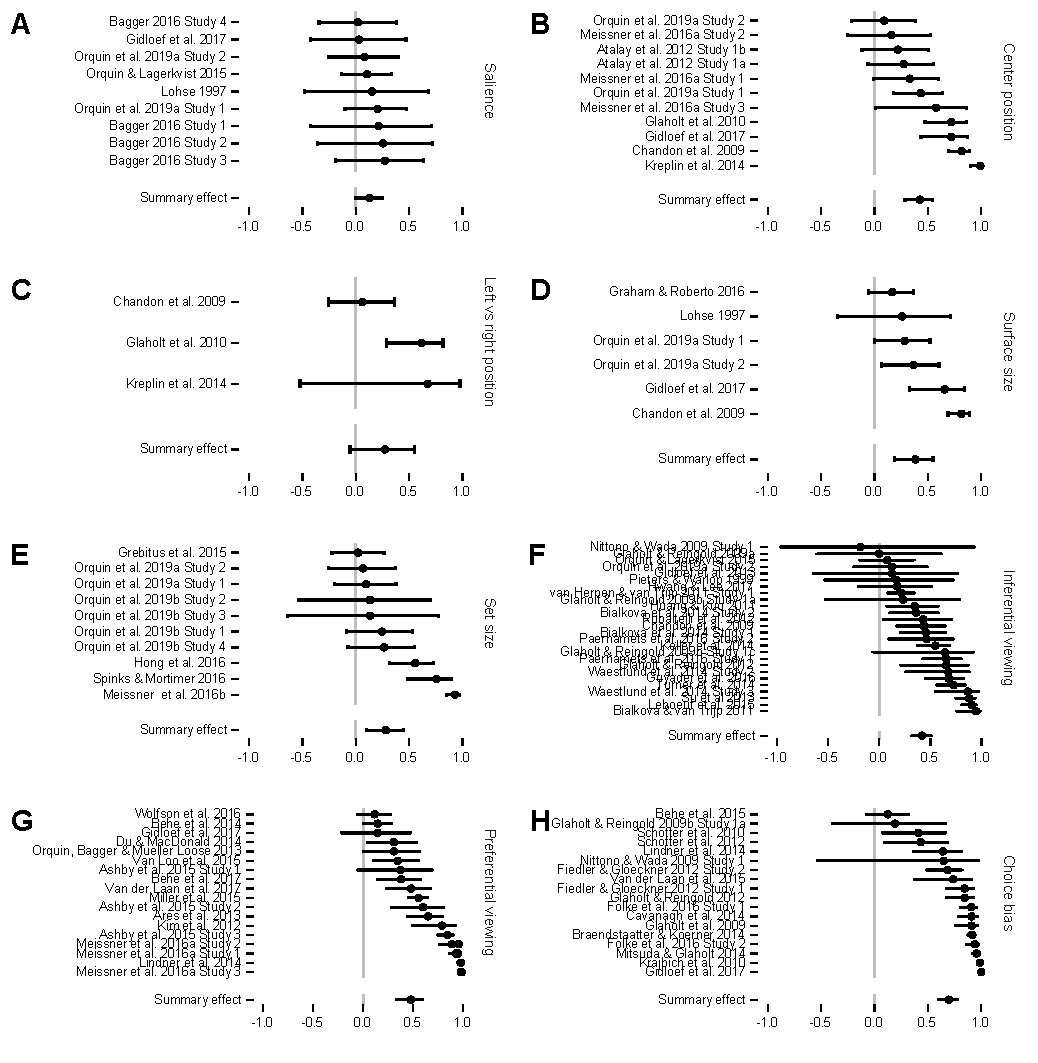
\includegraphics{forest_plots}
\centering
\caption{Forest plots showing the unattenuated effect size correlations for each study as well as average effect across study groups. Salience A), surface size B), left vs right position C), central position D), set size for alternative E), set size for attribute F), inferential viewing for alternative G), inferential viewing for attribute H), preferential viewing for alternative I), preferential viewing for attribute J), choice bias K). Error bars represent the 95\% confidence interval of the mean.}
\label{fig:forest_plots}
\end{figure}


\subsection{Publication bias}

We assessed potential publication bias using a trim-and-fill analysis (Duval \& Tweedie, 2000) of each subgroup. In addition, we plotted the Fisher $z$ transformed correlation coefficients of each study by its respective standard error (Figure~\ref{fig:funnel_plots}). The symmetry of the funnel plot in Figure~\ref{fig:funnel_plots} provides a qualitative picture of whether there is a file drawer problem, i.e. we expect that studies with smaller sample sizes and hence higher standard errors yield more variable effect sizes the smallest of which are less likely to be published leading to an asymmetric funnel plot. The trim-and-fill analysis resulted in a downward adjustment of the average effect size for most of the subgroups. The corrected effect sizes in Table~\ref{tab:trim_fill_results} provide a more conservative estimate of the true population effects, but are also subject to some uncertainty. Specifically, the interpretation of the corrected results may be biased due to heterogeneity in many of the subgroups as well as a relatively small number of studies in the bottom up factor groups.


\begin{figure}%[H]
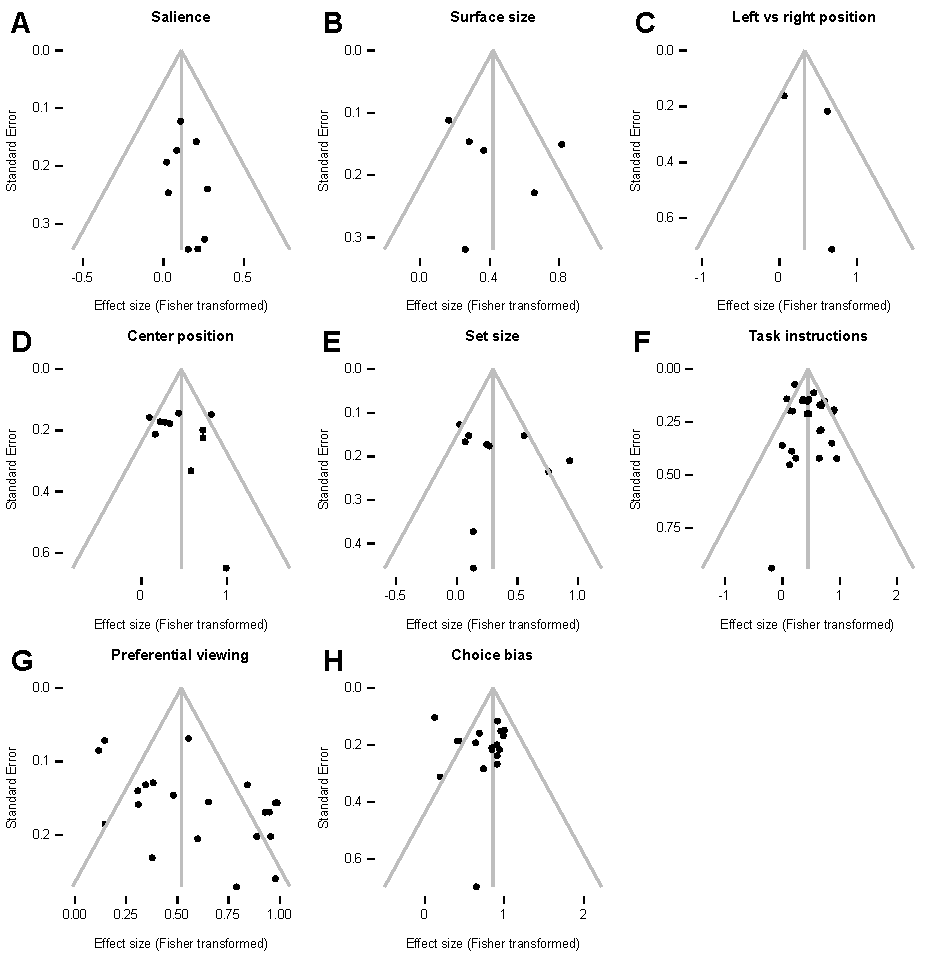
\includegraphics{funnel_plots}
\centering
\caption{Funnel plots for each study subgroup. Observations are Fishers z transformed correlation coefficients against their standard error. Asymmetric distributions of observations can indicate the presence of publication bias since smaller studies (those with higher standard errors) have more variable effect sizes and are less likely to be published unless the effect is large. Salience A), surface size B), left vs right position C), central position D), set size E), set size for alternative F), set size for attribute G), inferential viewing H), inferential viewing for alternative I), inferential viewing for attribute J), preferential viewing K), preferential viewing for alternative L), preferential viewing for attribute M), choice bias N).}
\label{fig:funnel_plots}
\end{figure}


% -------------------------------------------------------
% Discussion
% -------------------------------------------------------

\section{Discussion}

For the better part of our daily lives, we attend to and gather information using our eyes. We visually inspect food products in the supermarket or online, we read emails, task lists, memos, or software and spend considerable time looking at other people and our surroundings in an attempt to navigate our social and physical environment. Consequently, many of the decisions we make, small or large, are based on the visual information that we gather using our eyes. In this study, we attempt to answer how our eyes gather information during decision-making. We meta-analyze empirical studies on eye movements in decision-making and provide a quantitative overview of the factors driving eye movements in decision-making. We distinguish between internal or top-down factors such as preferential viewing, inferential viewing, and choice bias and external or bottom-up factors such as salience, surface size, set size, and position effects. We identify 107 effect sizes and perform a psychometric meta-analysis to control for issues related to the validity of each study. 


\subsection{Main findings}

Except for salience, $\rho = .15$, the results show that all bottom-up factors have medium to large effect sizes ranging from $\rho = .42$ to $\rho = .57$. In comparison, all three top-down factors are large, ranging from $\rho = .50$to $\rho = .77$, but not three times as large as previously hypothesized (Wedel \& Pieters, 2006). Considering that there is no bottom-up free visual environment, it is reasonable to expect that all bottom-up factors influence eye movements at the same time. In laboratory environments, it is possible, and often desirable, to control for bottom-up factors, but in natural environments where no such control or counterbalancing takes place, the visual environment could account for a large share of variance in eye movements. The mounting evidence that demonstrates a causal effect of eye movements on decision-making (Ghaffari \& Fiedler, 2018; Reeck et al., 2017; Pärnamets et al., 2015; Shimojo et al., 2003), therefore, suggest an important role for the visual environment in guiding our decisions through our eye movements. 

Regarding top-down factors, several findings have emerged. We decided to analyze studies on inferential viewing and preferential viewing separately since there is a clear qualitative difference between the two domains. In studies on inferential viewing, participants receive instructions concerning a specific decision goal, whereas, in preferential viewing studies, participants decide based on subjective preferences. The inspection of the effect sizes reveals that the main effect in the two types of studies are indistinguishable, i.e., similar effect sizes, $\rho$ task = .495 and $\rho$ preferential viewing  = .511 and overlapping credibility and confidence intervals. This result suggests that it makes no difference to eye movements whether the relevance of information is defined according to an externally specified goal or according to preferences. Breaking down both groups by moderators reveal further similarities. Both preferential viewing and inferential viewing are moderated by the subgroups alternatives and attribute, and in both cases, there is a larger effect at the alternative level. These findings dovetail with the moderation of set size where we also find a larger effect on set size by alternatives than set size by attributes. The result implies that decision-makers are more likely to adapt to increases in set size by ignoring alternatives than by ignoring attributes. One interpretation is that decision-makers are more oriented towards compensatory than non-compensatory decision rules, e.g., more likely to use satisficing than the lexicographic decision rules. 

Finally, we find that choice bias has a very large effect on eye movements. The choice bias effect is similar for preferential and inferential decision tasks, suggesting that eye movements are not driven by preferential viewing. Even in tasks where the chosen option is not the preferred option, decision-makers make more fixations to it. There could be several explanations for this finding. The choice bias might arise because of  a) the gaze cascade phenomenon (Shimojo et al., 2003), b) an evidence accumulation process as proposed to, for instance, the aDDM model (Krajbich, Armel, \& Rangel, 2010), c) coherence maximization as proposed in the parallel constraint satisfaction model (Glöckner \& Herbold, 2011), d) the result of a resource-rational process in which decision-makers prioritize attention (Callaway \& Griffiths, 2019), or e) a mere consequence of a preparations for a motor response towards the chosen option (Hayhoe \& Ballard, 2014). The specific mechanism behind choice bias remains unclear; but considering how large the effect is, and the number of models that imply this effect, we believe that a better, and eventually full understanding of the effect will help advance decision research. 


\subsection{Implications for other disciplines}

Our findings have implications for several scientific disciplines. We have focused our discussion on judgment and decision-making but will turn a few other topics. Our meta-analysis is, to the best of our knowledge, the first to quantitatively summarize findings on top-down and bottom-up control of eye movements in any discipline, including vision science. Naturally, other disciplines may want to take stock of these findings and have to evaluate the generalizability of the findings to their respective discipline. Since JDM is a broad term, several disciplines such as cognitive psychology, behavioral economics, and consumer psychology are represented in the set of included studies. For these disciplines, our findings provide a useful framework for developing choice architecture interventions (Münscher, Vetter, \& Scheuerle, 2016) based on bottom-up factors. Our findings also point to the possibility of measuring individual preferences in real time through eye movements – a technique that may become practically relevant once our devices have built-in eye trackers (Bulling \& Wedel, 2019).    

Given the high degree of variance in methodologies and stimuli, we expect that our results generalize well to other disciplines such as learning and education research, problem solving, or human-computer interaction. The disciplines studying eye movements in natural environments, e.g., driving, aviation, or other natural tasks, should be cautious when applying our findings since the vast majority of the included effect sizes were from laboratory-based studies. In general, our findings attest to an unexpectedly large influence of the visual environment on our eye movements. We believe that this pattern is likely to replicate in other disciplines as well.


\subsection{Methodological contributions}

So far, only a few meta-analyses have been published on eye movements, and no guidelines exist concerning how to deal with eye-tracking-specific issues in meta-analyses. To perform our analysis, we have developed procedures for how to handle issues related to multiple AOIs, multiple metrics, and eye tracker validity. The procedure for handling eye tracker validity showed that eye trackers with poorer accuracy, in general, lead to lower effect sizes. In our data, the difference in Ai between the best and worst eye trackers were spanning from .167 to .667. This result is a substantial difference. Accounting for eye tracker validity improved the precision of the synthesized effect sizes. This finding is, furthermore, an important methodological contribution which demonstrates the relevance of ensuring high-quality eye tracker data.

Regarding the multiple metrics such as fixation count, fixation likelihood, or dwell, count, we showed, first of all, that these metrics yield very similar effect sizes, and, second, that the effect sizes expressed in one metric can be converted to an effect size expressed in another metric. Regarding studies which report multiple AOIs, we propose to average the effect sizes across AOIs. An alternative would have been to weight the effect sizes depending on the relevance of the AOI to the research question, but this approach would have required precise and unambiguous predictions regarding the relevance of each AOI. Such precise predictions are rare but may become more frequent in the future since other researchers can now derive predictions based on our findings.   


\subsection{Limitations and future research}

Several limitations deserve to be mentioned. Most importantly, several of the bottom-up factors included a low number of studies which casts some doubt about the precision of the results. The low number of studies also analyzed the publication bias less reliable, thereby, adding to the uncertainty. Another challenge is that the studies included varied substantially because of stimulus differences, e.g., high vs. low complexity stimuli, and because of task differences, e.g., risky gambles vs. consumer decision-making. These differences may have introduced additional heterogeneity into the synthesized effect sizes, but at the same time, serve to increase the generalizability of the findings (Cooper, Hedges, \& Valentine, 2009). 

Our findings call into question several assumptions about how decision-makers search for and gather information. Several existing theories and models make assumptions that imply only a subset of the identified top-down and bottom-up factors. While these models may work in a controlled laboratory environment, it is clear that they do not generalize to more natural environments. Future models should, therefore, strive to incorporate a wide set of the identified factors to balance between top-down and bottom-up control. Another important avenue will be to gain a better understanding of the phenomenon of choice bias. How does it arise and what does it imply about the attention-choice process? From a methodological perspective, future research may further develop our framework for correcting for eye tracker accuracy. We know that several factors contribute to the validity of eye trackers, e.g., accuracy depends on the stimulus and the AOI size (Orquin \& Holmqvist, 2018) and other artifacts such as sample population and recording location also matter (Nyström, Andersson, \& Holmqvist, 2013). By extending our framework to include these other artifacts, it will be possible to make more precise estimates of effect sizes in meta-analysis and individual studies as well as more realistic power analyses.    


% -----------------------------------------------------------
% Method
% -----------------------------------------------------------

\section{Method}

\subsection{Literature Search}

Web of Science was searched using the following terms: eye track* OR eye move* OR eye fix* AND decision-making OR choice. Grey literature, such as reports and unpublished work, was identified in the first 2,000 hits on Google Scholar. No restrictions on publication date or language were imposed. Additional literature was identified by searching the reference lists of the identified papers and through contact with the authors. Calls for unpublished studies were distributed to the relevant research communities via email lists published February 2018 at the following lists; EADM, SJDM, and EGPROC. The search resulted in 291 studies screened for eligibility. The last search was done on March 1st, 2018.


\subsection{Inclusion Criteria}

We included studies in which participants made decisions or judgments between discrete alternatives while their eye movements were monitored using eye-tracking technology. We did not include studies related to perceptual judgments, such as categorizing or discriminating visual stimuli or studies on problem solving. We excluded studies where participants were selected based on clinical diagnosis or specific sociodemographic traits e.g., visual disorders, age-related visual diseases, age restrictions such as adolescents or infants. Studies using fixed exposure time or time pressure manipulations were excluded since these manipulations can influence eye movement processes (Orquin \& Holmqvist, 2018) and lead to different results (Simola, Kuisma, Kaakinen, 2019). Included studies used either fixation likelihood (AOI looked at or not), fixation count (number of fixations to AOI), total fixation duration (sum of durations of all fixation to an AOI), or dwell count (number of dwells to an AOI). Eventually, 58 articles met all inclusion criteria and were included in the meta-analysis (Figure~\ref{fig:flow_diagram}).



\subsection{Coding Procedure}

The included studies were coded with regards to their i) effect size, ii) sample size, iii) research domain, iv) eye tracker model, v) dependent variable, and vi) independent variable. All studies were initially coded by the first author and later by the second author. Any disagreement was resolved by discussion. Agreement for categorical variables was assessed using Cohen's kappa and for continuous variables using intraclass correlation coefficient (Shrout \& Fleiss, 1979). Overall, there was a high level of agreement: effect size, $\textrm{ICC} = 0.923$, sample size, $\textrm{ICC} = 0.996$, research domain, $\textrm{ICC} = 0.731$, eye tracker model, $\textrm{ICC} = 1$, dependent variable, $\kappa = 0.923$, independent variable, $\kappa = 0.934$.%
%
\footnote{Most of the printed coding sheets were unfortunately lost while moving between offices. The inter coder reliability is therefore computed on 20 observations from the random coding sheets that were recovered.}

Coding of effect sizes is described in detail below and sample size was coded as the total number of participants in a study. The research domain was coded as preferential consumer choice, inferential consumer choice, preferential non consumer choice, inferential non consumer choice, and risky gambles. The research domain was later recoded for the analysis of choice bias in the following way: inferential consumer choice and inferential non consumer choice were recoded as inferential choice while the other three domains were coded as preferential choice. We coded the eye tracker model as the specific name of the eye tracking equipment used in the study, e.g. Tobii T2150 or Tobii T60, since different models from the same producer vary in measurement accuracy and precision. Information on each eye tracker model's accuracy and precision was identified through the equipment producers' websites. We coded the dependent variable as the specific eye tracking metric in which an effect size was reported. We coded the independent variable as bottom-up control and top-down control, with bottom-up control divided into five dimensions, visual salience, surface size, left vs right position, central position, and set size, and top-down control divided into three dimensions, inferential viewing, preferential viewing, and choice bias. We outline these categories in detail below. 

\paragraph{Visual salience.} We coded studies as visual salience if they operationalized one or more of the known dimensions of visual salience such as color, edge density, contrast, or motion (Itti \& Koch, 2001). Some studies failed to indicate the direction of the salience manipulation, i.e. high vs. low levels of salience. In such cases, we contacted the original author and asked for clarification.

\paragraph{Surface Size} We coded studies that manipulated the relative surface size of alternatives or attribute, e.g., small vs. large alternatives or attributes (Lohse, 1997). Some studies manipulated the number of product facings, i.e., the number of the same product on a supermarket shelf (Chandon et al., 2009). We coded such manipulation as a surface size manipulation. 

\paragraph{Left vs right and center position.} We coded studies that manipulated the left vs right position of alternatives or attributes in horizontal arrays as left vs right position (Kreplin et al., 2014). We coded studies that manipulated the centrality of alternative or attribute position in one or two-dimensional arrays as center position (Atalay et al., 2012, experiment 1A \& 1B; Meissner, 2016a).

\paragraph{Set size.} We coded studies as set size if they manipulated the number of alternatives or attributes in a given choice task, e.g., studying the effect of a two- vs. three-alternative choice task (Hong et al., 2016). We also coded whether the set size was manipulated at the level of the alternative or the attribute. 

\paragraph{Inferential viewing.} We coded studies on inferential viewing if they presented participants with identical stimuli under different task instructions, e.g., presented participants with the same choice alternatives under a preferential choice task vs. a healthy choice task (Orquin et al., 2019). We also coded whether the unit of analysis was at the level of the alternative or the attribute, i.e. whether AOIs contained alternatives or attributes. 

\paragraph{Preferential viewing.} We coded studies on preferential viewing if they measured the effect of preferences on eye movements. We also coded whether the unit of analysis was at the level of the alternative, e.g. when participants prefer one alternative over another because it is cheaper or has a better flavor (Gidlöf et al., 2017), or at the level of attributes, e.g. when price is more important than flavor (Meissner et al., 2016a). 

\paragraph{Choice bias.} We coded studies as choice bias if they reported the difference in eye movements between the chosen alternative and all other (not chosen) alternatives. Studies that operationalized choice bias in specific time windows, e.g., the first 500 msec after stimulus onset or last 500 msec prior to choice (Shimojo et al., 2003) were excluded. Based on the research domain we coded choice bias in two subgroups: preferential tasks where participants performed a preferential choice task, that is where participants were instructed to choose in accordance with their preferences (Schotter et al., 2010) and inferential tasks where participants were instructed to choose in accordance with a predetermined goal, such as choosing the healthiest option (Schotter et al., 2012).


\subsection{Construct validity of the dependent variable}

A possible concern in meta-analyses of eye movements is that the included studies use different eye trackers since data quality varies considerably across different eye-tracking equipment. Precision, which is the reliability of an eye tracker, can vary as much as from .005\degree root mean square in the best to .5\degree in the poorest remote eye-trackers (Holmqvist et al., 2015). Accuracy, which is the validity of an eye tracker, vary from around .4\degree to around 2\degree (Holmqvist et al., 2015). With an accuracy of 2\degree, the measured fixation, will on average fall as far as 2\degree away from the true fixation point. Simulations have shown that both accuracy and precision influence the capture rate, i.e., the percentage of eye movements correctly recorded within the boundaries of stimuli, which determines the degree of false positive and false negative observations (Orquin \& Holmqvist, 2018, 2019). The level of false positive vs. negative fixations has been shown to influence effect sizes (Orquin, Ashby, \& Clarke, 2016). These differences in measurement validity across eye trackers may therefore introduce a bias in the meta-analysis of eye movements, since studies with lower accuracy and precision have lower validity, which, on average, attenuate effect sizes (Hunter \& Schmidt, 2004). To inspect whether the precision and validity of eye tracker attenuate effect sizes, and potentially correct for this, we ran a regression analysis on all included effect sizes with the absolute observed effect size correlation as the dependent variable and reported precision and accuracy of the eye tracking equipment as the independent variables. We fitted different models using a step-up approach based on AIC and BIC, including models with a fixed effect for the independent variable type (salience, surface size etc.). The final model included the main effect of accuracy and a random intercept grouped by study. The second-best model also included a fixed effect for independent variable type, and the estimates of the two models were comparable.

The accuracy and precision of eye trackers are highly correlated ($r = .63$), and presumably for this reason model fit did not improve when including precision. Despite analyzing across different study subgroups and other sources of noise, the results suggest that studies using eye trackers with lower levels of accuracy, on average, yield lower effect sizes as predicted by the psychometric meta-analysis methods, $\beta_0 = 0.569$, $\SE = 0.09$, $t = 6.293$, $p < .001$, $\beta_{\textrm{accuracy}} = -0.382$, $\SE = 0.158$, $t = -2.422$, $p = .018$, (Figure~\ref{fig:metric_correction}). Having demonstrated that the accuracy of eye trackers attenuates effect sizes, the next step is to correct for this phenomenon. Psychometric meta-analysis offers a method for correcting the attenuating effects of artifacts, such as the lack of validity or reliability. The correction involves an artifact multiplier, $a_a$, which is a measure of the expected attenuation of the true effect size $\rho$ caused by the artifacts in study $i$. The observed study effect size $\rho_0$ is a function of the true effect size and the artifact multiplier, $\rho_0 = a_a \rho$. In the case of measurement validity, the artifact multiplier is the square root of the validity of the measurement, $a_a = \sqrt{r_{yy}}$. From this calculation, it follows that the artifact multiplier, and, hence the validity of the measurement, can be obtained as $a_a = \rho_0 / \rho$ (Hunter \& Schmidt, 2004) From our model, we have estimated the observed attenuated effect size, $\rho_0$, of study $i$ as $\beta_0 + \beta_1 \textrm{accuracy}$. Given perfect accuracy, i.e. accuracy takes the value zero, the expected effect size of study i is equal to the intercept, $\beta_0$, which corresponds to the expected unattenuated effect size, $\rho$. From this it follows that the artifact multiplier, $a_a$, can be computed as the ratio of the attenuated effect size proportional to the unattenuated effect size:
%
\begin{equation}
\label{eq:artifact_multiplier}
a_a = \frac{\beta_0 + \beta_1 \textrm{accuracy}}{\beta_0}
\end{equation}

For example, if a study uses an eye tracker with an accuracy of $.50$, this yields an artifact multiplier equal to $(.66 – .553*.50)/.66 = .581$, meaning that studies with this level of accuracy will, on average, experience effect sizes that are $58.1\%$ of the true population effect size $\rho$. To compute the true average effect, $\rho$, we follow the psychometric meta-analysis method proposed by Hunter and Schmidt (2004). We first compute the unattenuated effect size correlation for each study, $r_i^u$, by dividing the Fisher $z$ transformed attenuated effect size with the artifact multiplier that corresponds to the level of the eye tracker accuracy and then applying the inverse Fisher transformation, $r_i^u = \tanh(\arctanh(r_i)/a_a)$. Then, we weight each study by its sample size and its level of validity, so that studies using low accuracy eye trackers are corrected upwards, in terms of their effect sizes and variance (see Equation~\ref{eq:psychometric_rho}). A full list of eye trackers and their accuracy and precision can be found in Appendix~\ref{appendix}.


\subsection{Multiple metrics}

A second methodological issue in meta-analyses of eye movements is that studies often rely on different eye movement metrics as their dependent variable. However, to perform a meta-analysis, we need to compare studies across a common dependent variable. The many different eye-movement metrics stem from different research designs and research questions and, perhaps, also a lack of consensus about when and why to use which metrics. Many studies on bottom-up factors report fixation likelihood while studies on top-down factors often report fixation or dwell count. We focus on fixation likelihood and fixation count since they are easier to interpret than both the total fixation duration and the dwell count. The total fixation duration can, for instance, be difficult to interpret when there is a correlation between the fixation duration and the fixation count (Orquin \& Holmqvist, 2018, 2019). The dwell count is similarly difficult to interpret if there is a correlation between the number of or the duration of fixations per dwell and the probability of a dwell. In order to inspect whether it would be meaningful to average effect sizes across different eye tracking metrics, we reviewed the identified articles for studies that reported effect sizes in multiple metrics. We identified in total $43$ studies reporting fixation likelihood along with one additional metric and $48$ studies reporting fixation count along with one additional metric. To investigate the strength of the relationship between metrics, we inspected the linearity of the relationship between fixation likelihood and fixation count against other metrics by plotting all observations (Figure~\ref{fig:metric_correction}). Since the four eye movement metrics are highly correlated, we assume that the metrics related to the same underlying construct. 

While effect sizes expressed in different metrics are highly correlated, we should expect some differences between them. One mechanism that could lead to differences in effect size estimates between fixation likelihood and the remaining metrics is artificial dichotomization since fixation count, dwell count and total fixation duration are categorized as a binary outcome (fixated or not fixated). Artificial dichotomization of a naturally continuous variable attenuates correlations with other variables (Hunter \& Schmidt, 2004), and we should, therefore, expect effect sizes expressed in fixation likelihood to be somewhat smaller. Correcting for artificial dichotomization requires knowledge about the true distributional split. Since none of the included studies provide information about the true distributional split of the dichotomization and since we do not have access to all data sets, we are unable to compute the artifact multiplier as proposed by Hunter and Schmidt (2004). Furthermore, since the distributions of the eye tracking metrics either zero inflated normal distributed (total fixation duration) or Poisson distributed (fixation and dwell count), no such adjustments for dichotomization currently exist. Instead, we propose an empirically derived correction factor, am, to convert effect sizes expressed in one metric to another. We propose to estimate the correction factor based on our sample of studies reporting multiple metrics, by taking the ratio of the sample size weighted means expressed in the two metrics of interest:
%
\begin{equation}
\label{eq:metrics_correction}
a_m = \frac{\arctanh \left( \frac{\sum M_i^1 N_i}{\sum N_i} \right)}{\arctanh \left( \frac{\sum M_i^2 N_i}{\sum N_i} \right)}
\end{equation}
%
where $\arctanh \left( \frac{\sum M_i N_i}{\sum N_i} \right)$ is the Fisher $z$ transformed average effect size for metric $M^1$ and $M^2$ respectively weighted by sample sizes, $N$. The ratio is computed on the Fisher $z$ transformed effect sizes in order to meaningfully compare ratios across the whole range of correlations. For similar reasons, the correction factor is applied to Fisher $z$ transformed effect sizes which are then transformed back with the inverse Fisher transformation: $\tanh(\arctanh(r_i)*a_m)$. The method takes advantage of the fact that effect sizes from the same study expressed in different metrics control for all factors that could influence the ratio.    

As expected, we find that effect sizes reported in fixation likelihood are on average smaller than those reported in metrics that are not artificially dichotomized, i.e. fixation count, dwell count, and total fixation duration. An effect size estimate expressed in fixation likelihood is, for instance, $97.2\%$ of the effect expressed in fixation likelihood. SI Table~\ref{tab:metric_correction} shows an overview of the correction factor $a_m$ when correcting to fixation likelihood (all bottom-up studies) and fixation count (all top-down studies). The correction factor is applied to each individual study effect size, but not to the study variance. When a study effect size is reported in the desired metric, e.g., fixation count for top-down studies, $a_m$ takes the value $1$.  


\subsection{Computation of effect sizes}

Effect size information was transformed into a common effect size, the Pearson’s correlation coefficient r using the R package compute.es (Del Re, A. C., \& Del Re, M. A., 2012). When multiple sources for computation of effect sizes were available, priority was given in decreasing order to other effect size measures such as eta squared, chi square, or odds ratio, means, and standard deviations, test statistics (e.g., F, t, wald), beta coefficient, or p values. For studies reporting effect sizes as correlations, no further computations were performed. If a study reported p values as a threshold value, e.g., $p < .05$, we used a conservative p value equal to .05. When studies reported effect sizes for multiple AOIs, we computed the average effect size across AOIs (for a similar approach, see Chita-Teigmark, 2016). Effect sizes were extracted from the available dependent variables. 


\subsection{Weighting of effect sizes, tests of heterogeneity}

The effect sizes were analyzed with a psychometric meta-analysis following the Hunter and Schmidt approach. Individual effect sizes were first corrected using the metric correction factor, $a_m$, to yield a common dependent variable. Studies on bottom-up factors were corrected to fixation likelihood, and studies on top-down factors were corrected to fixation count. The psychometric meta-analysis computes the true average effect size $\rho$ based on the unattenuated correlation coefficients, $r_i^u$, weighted by sample size $n_i$, and corrected for validity by the artifact multiplier, $a_a$: 
%
\begin{equation}
\label{eq:psychometric_rho}
\rho = \frac{\sum_{i=1}^k n_i a_a^2 r_i^u}{\sum_{i=1}^k n_i a_a^2}
\end{equation}

To inspect the degree of heterogeneity in the meta-analysis, we computed the $I^2$ statistic. The $I^2$ is the proportion of variance in the observed (attenuated) effect estimates explained by artifacts and sampling error (Borenstein et al. 2011): 
%
\begin{equation}
\label{eq:i2_statistic}
I^2 = \frac{(T^u)^2}{(S^u)^2}
\end{equation}
%
where $(S^u)^2$ is the weighted variance of the unattenuated effect size $\rho$
%
\begin{equation}
\label{eq:Su2_var}
(S^u)^2 = \frac{\sum_{i=1}^k n_i a_a^2 (\rho_i - \hat{\rho})^2}{\sum_{i=1}^k n_i a_a^2}
\end{equation}
%
and $(T^u)^2$ is the between-studies variance component of the unattenuated effect size $\rho$
%
\begin{equation}
\label{eq:Tu2_var}
(T^u)^2 = (S^u)^2 \frac{\sum_{i=1}^k n_i a_a^2 v_i}{\sum_{i=1}^k n_i a_a^2}
\end{equation}
%
where $v_i$ is the variance of study $i$ computed as $(1 - \hat{r}^2)^2 / (n_i - 1)$ and $\hat{r}$ is the sample size weighted average effect size.



% -----------------------------------------------------------
% Bibliography
% -----------------------------------------------------------

\bibliographystyle{apalike}
\bibliography{references.bib}



% -----------------------------------------------------------
% Appendix
% -----------------------------------------------------------

\section{Appendix}
\label{appendix}
\FloatBarrier


\begin{figure}
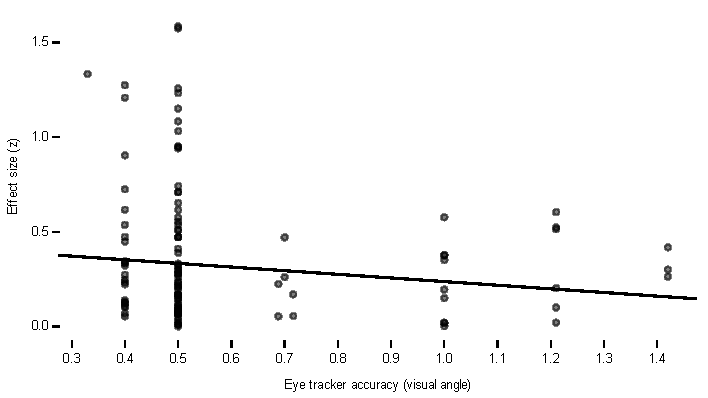
\includegraphics{ET_accuracy_effectsize}
\centering
\caption{Scatterplots showing the relationship between eye tracker accuracy and absolute effect size, estimated intercept and slope from the model were used to compute artifact multiplier (winning model).\hs{we need to update this description...perhaps add intercept and slope numbers to the figure?}}
\label{fig:ET_accuracy_effectsize}
\end{figure}
\clearpage


% \caption{Eye tracker specifications table}
% \label{tab:eyetracker_specs}
% latex table generated in R 3.5.2 by xtable 1.8-4 package
% Mon Nov 30 09:54:56 2020
\begin{table}[ht]
\centering
\caption{Eye tracker specifications table, with accuracy and precision for each eye tracker as extracted from the manufacturer website, and computed artifact multiplier used for correcting for a bias in effect size estimates.} 
\label{tab:eyetracker_specifications}
\begin{tabular}{lccc}
  \hline
Eye tracker model & $a_a$ & Accuracy & Precision \\ 
  \hline
ASL6000 & 0.5523 & 1.00 & 0.50 \\ 
  Easygaze & 0.6866 & 0.70 & 0.35 \\ 
  Eye gaze 97 & 0.6794 & 0.72 & 0.50 \\ 
  Eye gaze tm & 0.8209 & 0.40 & 0.50 \\ 
  EyeLink 1000 & 0.7762 & 0.50 & 0.05 \\ 
  EyeLink 1000 (acc = .33) & 0.8523 & 0.33 & 0.05 \\ 
  EyeLink 1000 Plus (acc < .5) & 0.7762 & 0.50 & 0.05 \\ 
  EyeLink II & 0.7762 & 0.50 & 0.01 \\ 
  ISCAN & 0.5523 & 1.00 & 0.50 \\ 
  Nihon-Kohden EEG-1100 & 0.5523 & 1.00 & 0.50 \\ 
  SMI Glasses & 0.4583 & 1.21 & 0.19 \\ 
  SMI RED & 0.8209 & 0.40 & 0.03 \\ 
  SMI iview & 0.7762 & 0.50 & 0.01 \\ 
  SMI iview HED & 0.5523 & 1.00 & 0.50 \\ 
  SMI model unknown (acc < .5) & 0.7762 & 0.50 & 0.30 \\ 
  Tobii D10 & 0.7762 & 0.50 & 0.50 \\ 
  Tobii Glasses 1 & 0.3643 & 1.42 & 0.50 \\ 
  Tobii T120 & 0.8209 & 0.40 & 0.24 \\ 
  Tobii T1750 & 0.7762 & 0.50 & 0.25 \\ 
  Tobii T2150 & 0.7762 & 0.50 & 0.35 \\ 
  Tobii T60 & 0.7762 & 0.50 & 0.22 \\ 
  Tobii X1 & 0.7762 & 0.50 & 0.20 \\ 
  Tobii X2 & 0.8209 & 0.40 & 0.32 \\ 
  Tobii X60 & 0.7762 & 0.50 & 0.30 \\ 
  Tobii glasses 2 & 0.3643 & 1.42 & 0.34 \\ 
  Unknown & 0.6919 & 0.69 & 0.30 \\ 
   \hline 
 \multicolumn{4}{l}{\scriptsize{\textit{Note.} $a_a$ = artifact multiplier.}} 
\end{tabular}
\end{table}

\clearpage


\begin{figure}%[H]
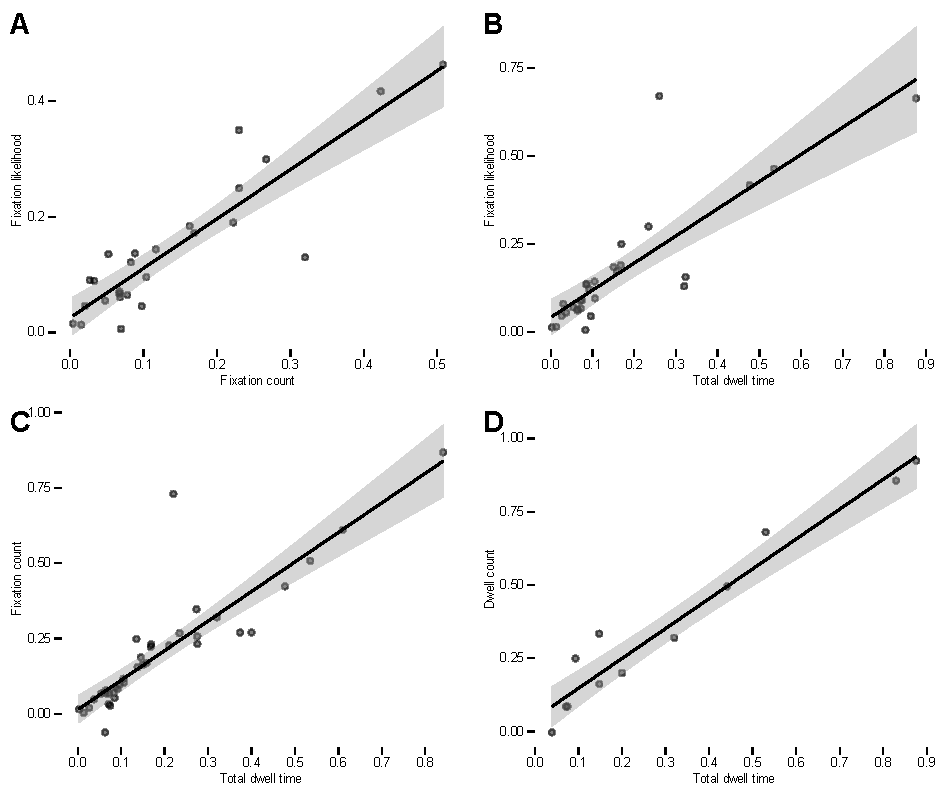
\includegraphics{metric_correction}
\centering
\caption{Scatterplots showing the relationship between effect sizes expressed in fixation likelihood and fixation count A), between total fixation duration and fixation likelihood B), between total fixation duration and fixation count C), between total fixation duration and dwell count D). The trend line in each plot represents the best-fitting linear regression line, and the shaded area around the trend line its 95\% confidence interval.}
\label{fig:metric_correction}
\end{figure}
\clearpage


% \caption{Metric correction factor $a_m$ when correcting to either fixation count or fixation likelihood}
% \label{tab:metric_correction}
% latex table generated in R 3.6.3 by xtable 1.8-4 package
% Fri Dec 18 00:07:07 2020
\begin{table}[ht]
\centering
\caption{Metric correction factor $a_m$ when correcting to either fixation count or fixation likelihood. These correction factors were used to make sure all dependent variables are comparable.} 
\label{tab:metric_correction}
\begin{tabular}{llc}
  \hline
Correcting from & Correcting to & $a_m$ \\ 
  \hline
Fixation count & Fixation likelihood & 1.041 \\ 
  Fixation likelihood & Fixation count & 0.961 \\ 
  Total dwell time & Fixation likelihood & 0.913 \\ 
  Total dwell time & Fixation count & 1.035 \\ 
  Dwell count & Fixation likelihood & 0.844 \\ 
  Dwell count & Fixation count & 0.957 \\ 
   \hline
\end{tabular}
\end{table}

\clearpage


% \caption{Trim and fill analysis for each independent subgroup.}
% \label{tab:trim_fill_results}
% latex table generated in R 3.6.3 by xtable 1.8-4 package
% Tue Jun 16 09:48:00 2020
\begin{table}[ht]
\centering
\caption{Trim and fill analysis for each visual and cognitive factor, including sub-factors used in the moderator analyses.} 
\label{tab:trim_fill_results}
\begin{tabular}{lccccccc}
  \hline
Group & Studies filled & $\rho$ & SE & $Z$ & $p$ & $\textrm{CI}_{95}$ LL & $\textrm{CI}_{95}$ UL \\ 
  \hline
\textbf{Visual factors} &  &  &  &  &  &  &  \\ 
  Salience & 2 & 0.111 & 0.063 & 1.766 & 0.077 & -0.012 & 0.233 \\ 
  Surface size & 0 & 0.384 & 0.108 & 3.562 & 0.000 & 0.173 & 0.595 \\ 
  Left vs right position & 2 & 0.061 & 0.223 & 0.273 & 0.785 & -0.376 & 0.497 \\ 
  Center position & 3 & 0.322 & 0.094 & 3.437 & 0.001 & 0.138 & 0.506 \\ 
  Set size & 0 & 0.282 & 0.098 & 2.887 & 0.004 & 0.090 & 0.473 \\ 
  \hspace{2mm}\textit{Alternative} & 1 & 0.459 & 0.105 & 4.376 & 0.000 & 0.253 & 0.665 \\ 
  \hspace{2mm}\textit{Attribute} & 0 & 0.137 & 0.116 & 1.175 & 0.240 & -0.091 & 0.365 \\ 
  \textbf{Cognitive factors} &  &  &  &  &  &  &  \\ 
  Task instruction & 3 & 0.384 & 0.065 & 5.947 & 0.000 & 0.257 & 0.510 \\ 
  \hspace{2mm}\textit{Alternative} & 1 & 0.544 & 0.072 & 7.579 & 0.000 & 0.403 & 0.685 \\ 
  \hspace{2mm}\textit{Attribute} & 2 & 0.355 & 0.085 & 4.189 & 0.000 & 0.189 & 0.521 \\ 
  Preferential viewing & 7 & 0.372 & 0.094 & 3.976 & 0.000 & 0.189 & 0.555 \\ 
  \hspace{2mm}\textit{Alternative} & 2 & 0.626 & 0.115 & 5.453 & 0.000 & 0.401 & 0.852 \\ 
  \hspace{2mm}\textit{Attribute} & 5 & 0.318 & 0.103 & 3.082 & 0.002 & 0.116 & 0.520 \\ 
  Choice bias & 7 & 0.490 & 0.094 & 5.225 & 0.000 & 0.306 & 0.674 \\ 
   \hline 
 \multicolumn{8}{p{0.9\textwidth}}{\scriptsize{\textit{Note.} $\rho$ = unattenuated effect size estimate, SE = standard error of estimate; $Z$ = Z statistic; $p$ = significance level; $\textrm{CI}_{95}$ LL = lower limit of the 95\% confidence interval; $\textrm{CI}_{95}$ UL = upper limit of the 95\% confidence interval. Italicized groups are moderator subgroups.}} 
\end{tabular}
\end{table}

\clearpage


\begin{figure}%[H]
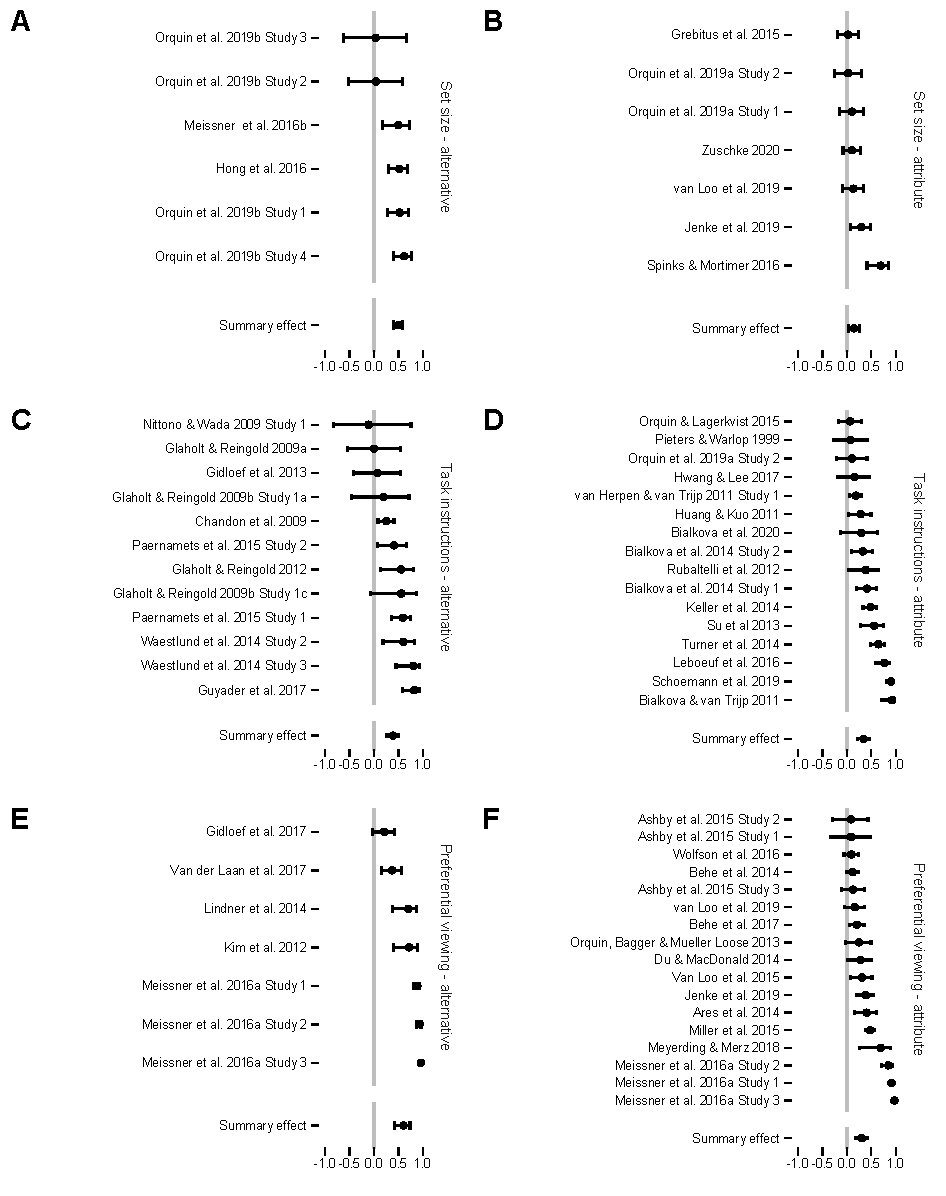
\includegraphics{forest_plots_altatt}
\centering
\caption{Forest plots showing the unattenuated effect size correlations for each study as well as average effect across study groups. Salience A), surface size B), left vs right position C), central position D), set size for alternative E), set size for attribute F), inferential viewing for alternative G), inferential viewing for attribute H), preferential viewing for alternative I), preferential viewing for attribute J), choice bias K). Error bars represent the 95\% confidence interval of the mean.}
\label{fig:forest_plots_altatt}
\end{figure}
\clearpage


\begin{figure}%[H]
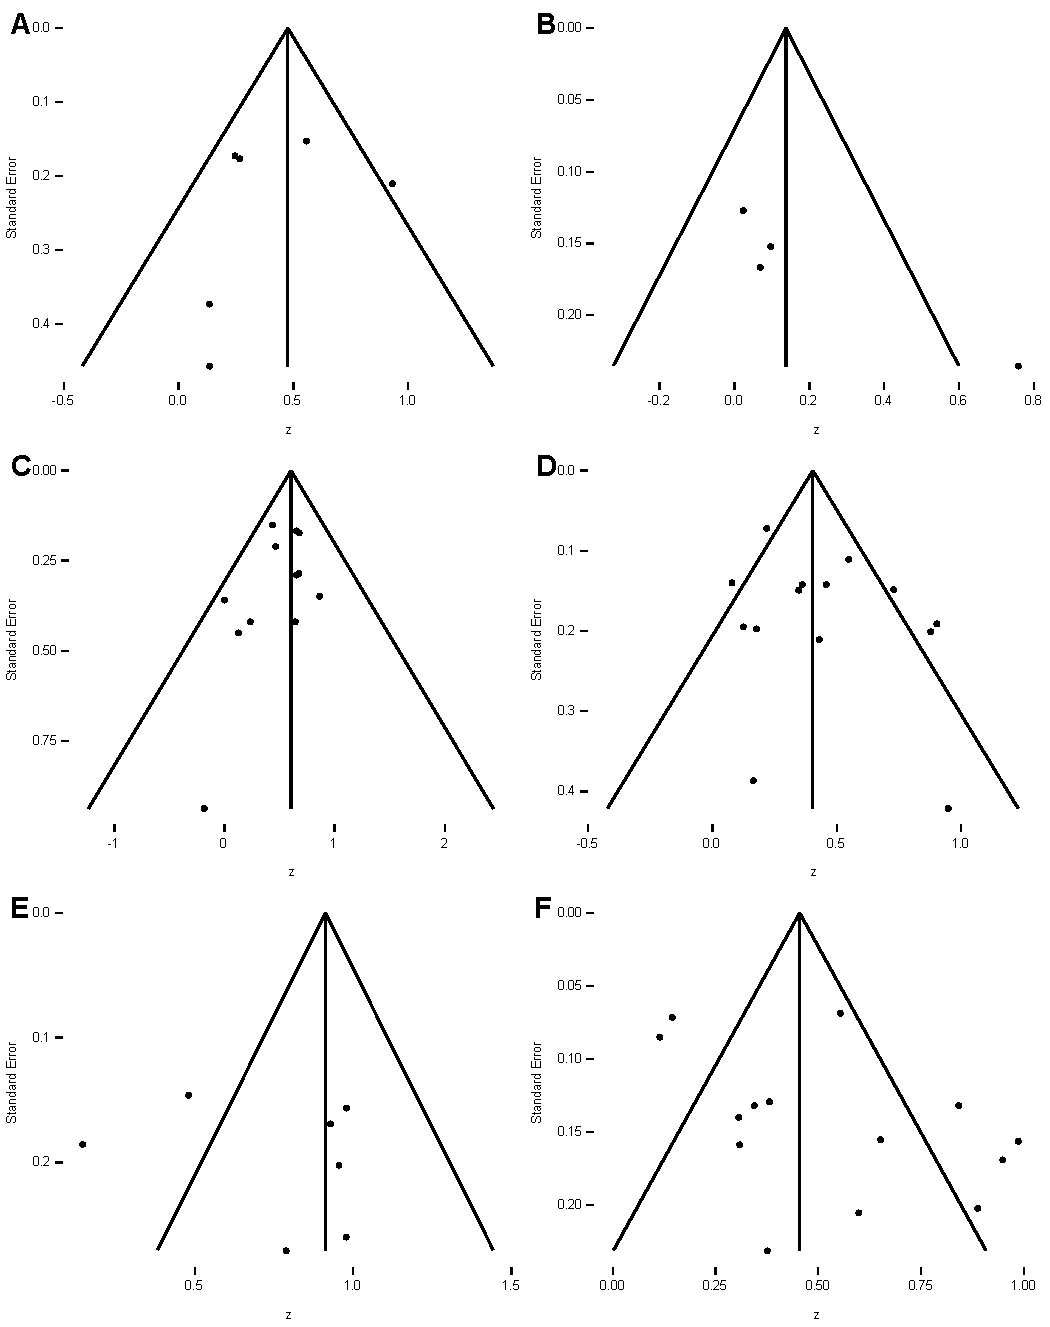
\includegraphics{funnel_plots_altatt}
\centering
\caption{Funnel plots for each study subgroup. Observations are Fishers z transformed correlation coefficients against their standard error. Asymmetric distributions of observations can indicate the presence of publication bias since smaller studies (those with higher standard errors) have more variable effect sizes and are less likely to be published unless the effect is large. Salience A), surface size B), left vs right position C), central position D), set size E), set size for alternative F), set size for attribute G), inferential viewing H), inferential viewing for alternative I), inferential viewing for attribute J), preferential viewing K), preferential viewing for alternative L), preferential viewing for attribute M), choice bias N).}
\label{fig:funnel_plots_altatt}
\end{figure}
\clearpage


\end{document}